\documentclass{beamer}
% \usepackage[utf8]{inputenc}
\usepackage[T1]{fontenc}
\usetheme{CambridgeUS}
\useoutertheme{miniframes}
\usecolortheme{dove}
\usefonttheme{serif}
\beamertemplatenavigationsymbolsempty

\usepackage[english]{babel}
% \usepackage[english, polish]{babel}

\usepackage{listings}
\lstset{basicstyle=\ttfamily\footnotesize,breaklines=true}
\usepackage{siunitx}
\usepackage{mhchem}
\usepackage{pifont}
\usepackage{amsmath,amssymb,amsfonts}
\usepackage{graphicx}
\usepackage[export]{adjustbox}
\usepackage{float}
\usepackage{xcolor}
\usepackage{setspace}

\newcommand{\todo}[1]{\textcolor{red}{TODO: #1}}

\newcommand{\imagesource}[1]{
    \begin{spacing}{0.5}
        \texttt{\textit{ \tiny{source: #1}}}
    \end{spacing}
}

\newenvironment{columnframe}[1]{
    \begin{frame}[environment=columnframe,fragile]{#1}
        \begin{columns}
            }{
        \end{columns}
    \end{frame}
}


\title{Enhanced Radars}
    \subtitle{and curious properties of Rydberg Atoms}
\author{Tobiasz Fic}
\date{28 May 2024}

\begin{document}

\begin{frame}
    \maketitle
    \begin{figure}
        \centering
        
\includegraphics[width=0.6\textwidth]{images/logo_eng.png}
    \end{figure}
\end{frame}

\begin{columnframe}{RADAR 101}
    \begin{column}{0.5\textwidth}
        \begin{figure}
            \centering
            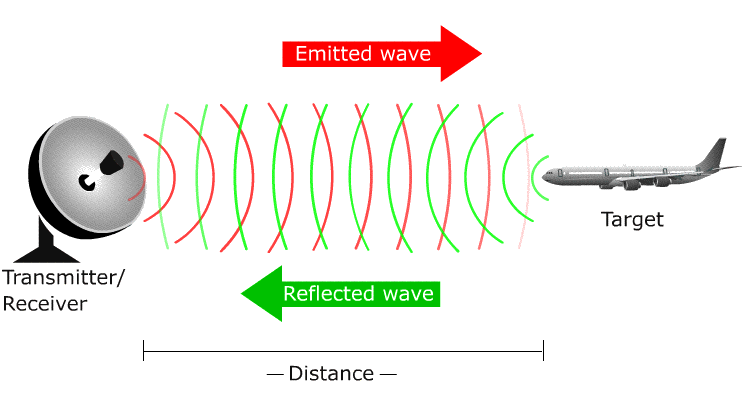
\includegraphics[width=\textwidth]{images/radar_demo.png}
        \end{figure}
    \end{column}
    \begin{column}{0.5\textwidth}
        \begin{itemize}
            \item In one sentence: send an RF signal, measure the time it takes to return, then calculate the distance.
            \item Precision is heavily dependent on our ability to measure sub-quantities.
        \end{itemize}
    \end{column}
\end{columnframe}

\begin{columnframe}{What can we use radars for?}
    \begin{column}{0.5\textwidth}
        \begin{figure}
            \centering
            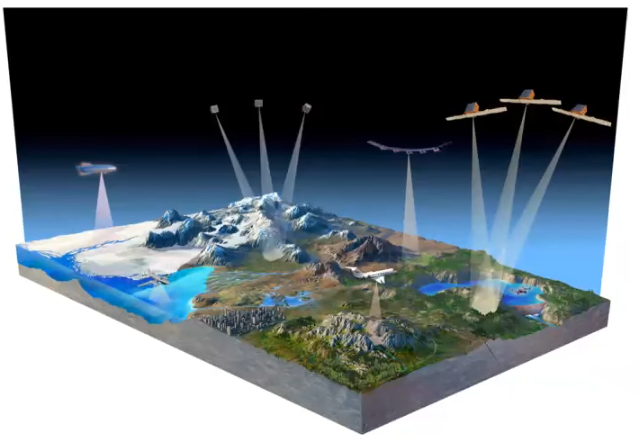
\includegraphics[width=\textwidth]{images/satellite_demo.png}
        \end{figure}
    \end{column}
    \begin{column}{0.5\textwidth}
        \begin{itemize}
            \item Originally: military applications
            \item Nowadays: weather forecasting, air traffic control, speed cameras, land surveying, etc.
        \end{itemize}
    \end{column}
\end{columnframe}



\begin{frame}{Conventional RF sensing}
    \begin{columns}
        \begin{column}{0.5\textwidth}
            \begin{itemize}
                \item The simplest RF sensor is a dipole antenna - turning electric field disturbances into voltage
                \item Notoriously difficult to calibrate
                \item Made of metal, so they interfere with the signal
                \item Size is dependent on the frequency (some are huge!)
            \end{itemize}
        \end{column}
        \begin{column}{0.5\textwidth}
            \begin{figure}
                \centering
                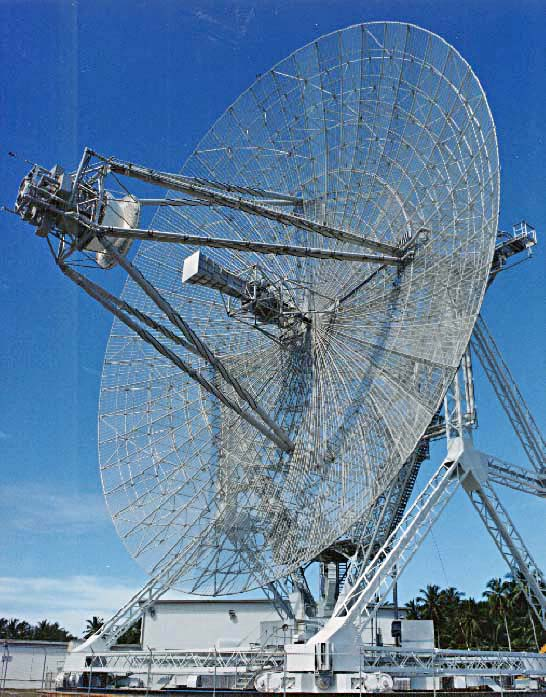
\includegraphics[width=0.8\textwidth]{images/radar_antenna_huge.jpg}
            \end{figure}
        \end{column}
    \end{columns}
\end{frame}

\begin{columnframe}{Curious properties of Alkali Metals}
    \begin{column}{0.5\textwidth}
        \begin{figure}
            \centering
            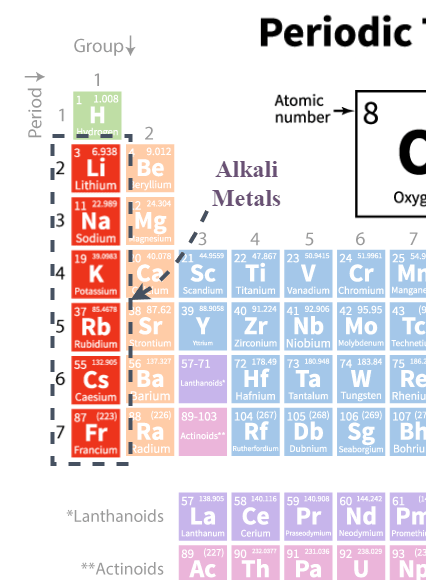
\includegraphics[width=0.8\textwidth]{images/alkali_metals_tb_of_elements.png}
        \end{figure}
    \end{column}
    \begin{column}{0.5\textwidth}
        \begin{itemize}
            \item Alkali metals only have one electron on the outermost shell
            \item They are easy to excite and predictable
            \item Lasers! (We like lasers: simple and precise)
        \end{itemize}
    \end{column}
\end{columnframe}

\begin{columnframe}{Rydberg atoms}
    \begin{column}{0.5\textwidth}
        \begin{figure}
            \centering
            
\includegraphics[width=0.6\textwidth]{images/pusheen.png}
        \end{figure}
    \end{column}
    \begin{column}{0.5\textwidth}
        \begin{itemize}
            \item A Rydberg atom is an atom in which the outer electron is in a highly excited state.
            \item Very sensitive to disturbances in the electric field.
            \item Tuned with lasers, read-out with lasers
            \item Alkali: $Cs^{55}$, or $Rb^{37}$
        \end{itemize}
    \end{column}
\end{columnframe}

\begin{columnframe}{Detecting RF radiation with Rydberg atoms}
    \begin{column}{0.5\textwidth}
        \begin{figure}
            \centering
            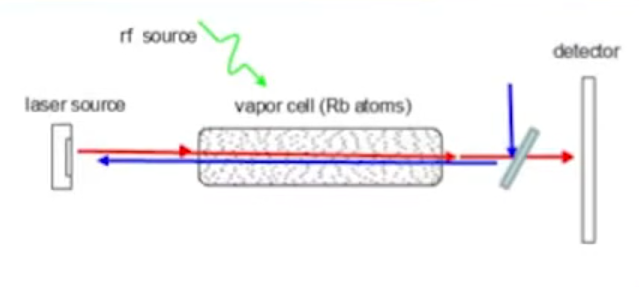
\includegraphics[width=0.8\textwidth]{images/detection_diagram.png}
        \end{figure}
    \end{column}
    \begin{column}{0.5\textwidth}
        \begin{itemize}
            \item Rydberg atoms are very sensitive to electric fields
            \item They are self-calibrating - properties are linked to fundamental constants
            \item Gas - no metal - no interference
            \item Stable quantum objects
            \item Large frequency range, no size change (tuned with lasers)
            \item Scalable/portable
        \end{itemize}
    \end{column}
\end{columnframe}

\begin{columnframe}{Measuring RF field intensity}
    \begin{column}{0.5\textwidth}
        \begin{figure}
            \centering
            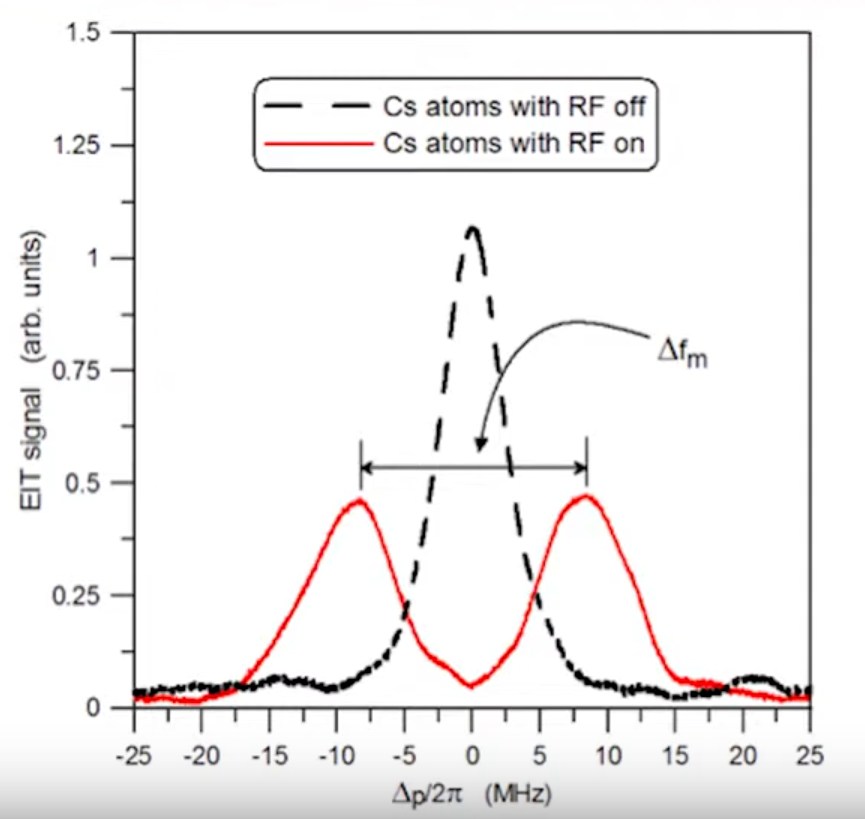
\includegraphics[width=\textwidth]{images/rydberg_eit.png}
        \end{figure}
    \end{column}
    \begin{column}{0.5\textwidth}
        \begin{itemize}
            \item A laser is directed at the atoms to excite them
            \item A second laser is directed the other way towards a detector to read out the results via
                  Electromagnetically-Induced transparency (EIT)
            \item Distance between peaks in frequency space corresponds to intensity of field of the tuned frequency
        \end{itemize}
    \end{column}
\end{columnframe}

\begin{columnframe}{Measuring RF field phase}
    \begin{column}{0.5\textwidth}
        \begin{figure}
            \centering
            
\includegraphics[width=0.6\textwidth]{images/pusheen.png}
        \end{figure}
    \end{column}
    \begin{column}{0.5\textwidth}
        \begin{itemize}
            \item one
            \item two
            \item three
        \end{itemize}
    \end{column}
\end{columnframe}

\begin{columnframe}{Repercussions}
    \begin{column}{0.48\textwidth}
        \begin{itemize}
            \item These new detectors can measure wide frequency spectrums (up to terahertz!)
            \item Radar accuracy will be increased
            \item Applications in Astronomy (RF telescope from space)
        \end{itemize}
    \end{column}
    \begin{column}{0.48\textwidth}
        \begin{itemize}
            \item one
            \item two
            \item three
        \end{itemize}
    \end{column}
\end{columnframe}

\begin{columnframe}{NIST: measuring standards}
    \begin{column}{0.48\textwidth}
        \begin{itemize}
            \item Electric field standards based only on Planck's constant
            \item Calibration becomes much easier
        \end{itemize}
    \end{column}
    \begin{column}{0.48\textwidth}
        \begin{itemize}
            \item one
            \item two
            \item three
        \end{itemize}
    \end{column}

\end{columnframe}

\begin{frame}{}
    \centering
    \Large{Thank you for your attention}
\end{frame}

\end{document}